\documentclass[12pt]{article}  

\usepackage
[colorlinks=true, pdfstartview=FitV, linkcolor=blue, citecolor=blue, urlcolor=blue]
{hyperref}

\usepackage{amssymb}  
\usepackage{amsthm}
\usepackage{amsmath}
\usepackage{graphics} 
\usepackage{graphicx} 
%\usepackage[latin1]{inputenc}
\usepackage{tikz}
\usepackage{pgfplots}
\usepackage{wrapfig}
\usepackage{caption}
\usepgfplotslibrary{polar}
\usepackage{ skull }


% GNUPLOT required
\usepackage{verbatim}

\linespread{1.3}

%\addtolength{\textwidth}{80pt}
\addtolength{\evensidemargin}{20pt}
\addtolength{\oddsidemargin}{20pt}

%%%%%%%%%%%%%%%%%%%%%%%%%%%%%%%%%%%%%%%%%%%%%%
%  Begin user defined commands

\newcommand{\map}[1]{\xrightarrow{#1}}

\newcommand{\N}{\mathbb N}
\newcommand{\Z}{\mathbb Z}
\newcommand{\Primes}{\mathbb P}
\newcommand{\Q}{\mathbb Q}
\newcommand{\R}{\mathbb R}
\newcommand{\C}{\mathbb C}
\newcommand{\bz}{\mathbb Z}
\newcommand{\bq}{\mathbb Q}
\newcommand{\br}{\mathbb R}
\newcommand{\bc}{\mathbb C}
\newcommand{\al}{\alpha}
\newcommand{\be}{\beta}
\newcommand{\ga}{\gamma}
\newcommand{\de}{\delta}
\newcommand{\ep}{\epsilon}
\DeclareMathOperator{\lub}{l.u.b.}
%  End user defined commands
%%%%%%%%%%%%%%%%%%%%%%%%%%%%%%%%%%%%%%%%%%%%%%


%%%%%%%%%%%%%%%%%%%%%%%%%%%%%%%%%%%%%%%%%%%%%%
% These establish different environments for stating Theorems, Lemmas, Remarks, etc.

\newtheorem{Thm}{Theorem}
\newtheorem{Prop}[Thm]{Proposition}
\newtheorem{Lem}[Thm]{Lemma}
\newtheorem{Cor}[Thm]{Corollary}

\theoremstyle{definition}
\newtheorem{Def}[Thm]{Definition}

\theoremstyle{remark}
\newtheorem{Rem}[Thm]{Remark}
\newtheorem{Ex}[Thm]{Example}

\theoremstyle{definition}
\newtheorem{Exercise}{Problem}

\newenvironment{Solution}{\noindent\textbf{Solution.}}{}
\newenvironment{Proof}{\noindent\textbf{Proof.}}{}
%\renewcommand{\labelenumi}{(\alph{enumi})}
\renewcommand\qedsymbol{QED}
% End environments 
%%%%%%%%%%%%%%%%%%%%%%%%%%%%%%%%%%%%%%%%%%%%%%%
%Some commands to save paper


\setlength{\parindent}{0in}
\setlength{\parskip}{8pt}

\DeclareMathOperator{\arcsec}{arcsec}
\DeclareMathOperator{\arccot}{arccot}
\DeclareMathOperator{\arccsc}{arccsc}
\DeclareMathOperator{\LH}{\ \underset{\text{LH}}{=}\ }
\newcommand{\Dep}{\Delta_+}
\newcommand{\Dem}{\Delta_-}
\newcommand{\bu}{\mathbf u}
\newcommand{\bv}{\mathbf v}
\newcommand{\bw}{\mathbf w}

\newcommand{\ora}{\overrightarrow}



\addtolength{\textwidth}{80pt}
\addtolength{\evensidemargin}{-40pt}
\addtolength{\oddsidemargin}{-40pt}
\addtolength{\topmargin}{-80pt}
\addtolength{\textheight}{1.8in}

\setlength{\parindent}{0in}
\setlength{\parskip}{8pt}

\DeclareMathOperator{\arcsinh}{arcsinh}

%%%%%%%%%%%%%%%%%%%%%%%%%%%%%%%%%%%%%%%%%%%%%%
% Now we're ready to start
%%%%%%%%%%%%%%%%%%%%%%%%%%%%%%%%%%%%%%%%%%%%%%

\begin{document}  

%\author{Your Name}
{\bf MATH 1103 Homework 1}\\
{\bf Due Friday January 26, 2018}

Practice Problems (not to be turned in)

\vskip5pt
{\bf Practice 1.\ } Use the $\ep$-lemma (section 2 of the notes) to prove the equality of decimals
\[.99999\dots=1.\]
\begin{Solution}
Set $x=.99999\dots$.  We know that $x\leq 1$. Suppose $x<1$. 
Let $\ep$ be an arbitrary positive number. Adding $\ep$ to $x$ will cause a $1$ to carry over to the left of the decimal point, so $1\leq x+\ep$. 
Therefore $ x< 1\leq x+\ep$, so $1-x<\ep$. By the $\ep$ theorem, we have $x=1$. 
\end{Solution}

{\bf Practice 2.\ } IIlustrate Archimedes' Series (see Introduction) 
\[\frac{3}{4}+\frac{3}{16}+\frac{3}{64}+\cdots=1,\]
using an equilateral triangle instead of a square. 

{\bf Practice 3.\ } (Warmup for the next page) Use Archimedes' formula for the area of a parabolic segment to compute the area of the region bounded by the graphs of $y=x^2$ and $y=2x+3$. 

(answer: $32/3$)

{\bf Practice 4.\ } Compute $\lim\limits_{n\to\infty}\dfrac{n}{2n+1}$, using algebra and a limit property. 

{\bf Practice 5.\ } Suppose $(x_n)$ is a sequence. 

a) Suppose $|x_n|\to 0$. Use a limit property to prove that $x_n\to 0$.

b)\ Suppose $x_n\to 0$. Use a limit property to prove that $|x_n|\to 0$.

\begin{Solution}

a)\ Squeeze Law, using $-|x_n|\leq x_n\leq |x_n|$. 

b)\ Define $b_n=|x_n|/x_n$ if $x_n\neq 0$, $b_n=0$ if $x_n=0$, 
so that $|x_n|=b_n\cdot x_n$. 
The sequence $b_n$ is bounded, and $x_n\to 0$. So $|x_n|\to 0$ by the Bounded-Times-Zero property. 

\end{Solution}

{\bf Practice 6.\ } (Challenging) Let $r$ any positive real number. 
Prove that 
\[\lim_{n\to\infty}\dfrac{r^n}{n!}=0.\] 

Hint: Choose an integer $p>r$ and show that for $n\geq p$ we have
\[\frac{r^n}{n!}\leq C\cdot \left(\frac{r}{p+1}\right)^n,\]
where $C$ is a constant depending only on $p$. 

\rule{\textwidth}{1pt}
The homework to be turned in may be found on the next page.
\newpage

{\bf Homework to be turned in}

{\bf 1.\ } Prove that $\dfrac{1}{\sqrt{n}}\to 0$ using $\ep$. 

\begin{Proof} 
Let $\ep$ be an arbitrary positive number. 
\newline
We must find an integer $N$ such that $\dfrac{1}{\sqrt{n}}<\ep$ for all integers $n\geq N$. 
\newline
Choose $N$ to be any integer such that $N> 1/\ep^2$. 
Then $\dfrac{1}{\sqrt{N}}<\ep$. 
\newline
Now if $n\geq N$ we have $\dfrac{1}{\sqrt{n}}\leq \dfrac{1}{\sqrt{N}}<\ep$. 
Therefore we have proved that  $\dfrac{1}{\sqrt{n}}\to 0$. 
\qed
\end{Proof}

\vskip10pt
{\bf 2.\ } Prove $\dfrac{\sin n}{n}\to 0$, using limit properties and what you know about the sine function. 

\begin{Proof} For all positive integers $n$ we have $-1\leq \sin n\leq 1$, so  
\[\frac{-1}{n}\leq \frac{\sin n}{n}\leq \frac{1}{n}.\]
We know $\pm 1/n\to0$, so by the Squeeze Law, 
\[\frac{\sin n}{n}\to 0\]
as well, as was to be shown. 
\end{Proof} 

\rule{\textwidth}{1pt}
The goal of the remaining five problems is to verify Archimedes' claim that the sum of all the vertex triangles in a parabolic segment equals four-thirds of the first vertex triangle. You will be using $(x,y)$-coordinates and algebra, plus a little bit of calculus (but not integration!). Archimedes proved his claim without such tools. 

In problem 3, you can use the following area formula without proof. Let 
$A=(a,a'),\  B=(b,b')$ and $ C=(c,c')$
be vertices of a triangle $ABC$ arranged so that when you move from $A$ to $B$ to $C$ you are going clockwise around the triangle $ABC$. Then the area of the triangle is given by
\[\text{area}(ABC)=\tfrac{1}{2}\left[(cb'-bc')+(ac'-ca')+(ba'-ab')\right].\]
\rule{\textwidth}{1pt}

{\bf 3.\ } Suppose $A=(a,a^2),\ B=(b,b^2),\ C=(c,c^2)$ are  points on the parabola $y=x^2$, arranged in clockwise order as above. 
Find the area of the triangle $ABC$ in terms of $a,b,c$. In your formula you should factor each of the three terms inside $[\cdots]$ in the area formula, because this will make later work simpler.

\begin{Solution} 
\[\begin{split}
\text{area}(ABC)
&=\tfrac{1}{2}\left[(cb^2-bc^2)+(ac^2-ca^2)+(ba^2-ab^2)\right]\\
&=\tfrac{1}{2}\left[bc(b-c)+ac(c-a)+ab(a-b)\right]
\end{split}
\]
\end{Solution} 

\vskip20pt
{\bf 4.\ }
Let $A=(a,a^2)$ and $B=(b,b^2)$ be two points on the parabola $y=x^2$, and assume now that  $C=(c,c^2)$ is the vertex of the segment cut off by the line $AB$. Recall $C$ is the point on the parabola where the tangent line is parallel to the line $AB$.
Compute $c$ in terms of $a$ and $b$. (It's ok to use derivatives.)

\begin{Solution} The slope of $AB$ is $a+b$ and the slope of tangent line at $C$ is $2c$, so $a+b=2c$, meaning that 
\[c=\frac{a+b}{2}.\]
\end{Solution} 



\vskip20pt


{\bf 5.\ }
Compute the area of the triangle $ABC$, for $A,B,C$ as in problem 4. Simplify your answer down to the cube of something involving just $a$ and $b$. 
\vskip5pt
\begin{Solution} Using the formula from Problem 1 with $c=(a+b)/2$, we have 
\[b-c=c-a=\frac{b-a}{2},\]
so 
\[\begin{split}
\text{area}(ABC)
&=\frac{1}{2}\left[
b\left(\frac{a+b}{2}\right)\left(\frac{b-a}{2}\right)
+a\left(\frac{a+b}{2}\right)\left(\frac{b-a}{2}\right)+ab(a-b)
\right]\\
&=\frac{b-a}{8}\left[b(a+b)+a(a+b)-4ab\right]\\
&=\frac{b-a}{8}\left[(a+b)^2-4ab\right]\\
&=\frac{b-a}{8}(b-a)^2\\
&=\left(\frac{b-a}{2}\right)^3
\end{split}
\]

\end{Solution}

\vskip20pt
{\bf 6.\ } Let $A,B,C$ be as in problem 4. 
Let $E$ be the vertex of the segment cut off by $AC$, and let $D$ be the vertex of the segment cut off by $CB$. Use your formula in problem 3 to show that 
\[\text{area}(ACE)+\text{area}(BCD)=\frac{1}{4}\text{area}(ABC).\]
\begin{center}
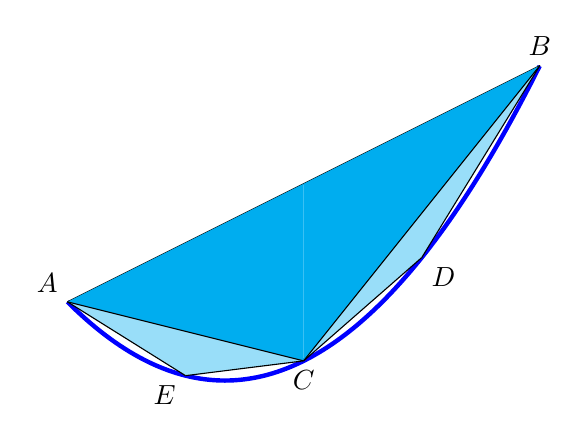
\begin{tikzpicture}[samples=100, domain=-1:2, scale=2]
\draw[ultra thick, color= blue]   plot (\x,{(\x*\x)/2})   node[right] {}; %parabola
\draw[-] (-1,.5) -- (2,2) node[right] {}; %secant AB
%\draw[thin, color=gray]   plot (\x,{(.5)*\x-.125})   node[right] {};%tangent
     \node[above left] at (-1,.5) {$A$};
     \node[above] at (2,2) {$B$};
     \node[below] at (.5,.125) {$C$}; %vertex
                    
   % \node[above left] at (.5,1.25) {$M$};
    %\fill[red!20] (-1,.5) -- (2,2) -- (.5,.125); %ABC
    \fill[cyan] (-1,.5) -- (.5,.125) -- (.5,1.25); %ACM
    \fill[cyan!40] (-1,.5) -- (.5,.125) -- (-.25,.031); %ACE
    %\fill[red] (-1,.5) -- (-.625,.195) -- (-.25,.031); %AFE
    %\fill[red]  (.125,.007) -- (.5,.125) -- (-.25,.031); %GCE
    \fill[cyan] (2,2) -- (.5,.125) -- (.5,1.25); %BCM
     \fill[cyan!40] (2,2) -- (.5,.125) -- (1.25,.781); %BCD
      %\fill[red] (7/8,49/128) -- (.5,.125) -- (1.25,.781); %HCD
      %\fill[red] (2,2) -- (13/8,169/128) -- (1.25,.781); %BID
       \draw[-] (-1,.5) -- (.5,.125); %AC
        \draw[-] (.5,.125) -- (2,2) ; %BC

      %\draw[-] (.5,.125) -- (.5,1.25) ; %CM
        \draw[-] (.5,.125) -- (1.25,.781) ; %CD
        \draw[-] (1.25,.781) -- (2,2) ; %DB
    \node[below right] at (1.25,.781) {$D$};
        \draw[-] (-1,.5) -- (-.25,.031); %AE
        \draw[-] (.5,.125) -- (-.25,.031); %CE     
    \node[below left] at (-.25,.031){$E$};
\end{tikzpicture}
\end{center}

\begin{Solution} From problem 5 we have 
\[\text{area}(ABC)=\left(\frac{b-a}{2}\right)^3,\qquad
\text{area}(ACD)=\left(\frac{c-a}{2}\right)^3,\qquad 
\text{area}(BEC)=\left(\frac{b-c}{2}\right)^3.
\]
Since $c=(a+b)/2$ we have $c-a=b-c=(b-a)/2$, so 
\[
\text{area}(ACD)=\text{area}(BEC)=\left(\frac{b-a}{4}\right)^3=\frac{1}{8}\left(\frac{b-a}{2}\right)^3
\]
so 
\[\text{area}(ACD)+\text{area}(CBE)=\frac{1}{4}\text{area}(ABC),\]
as desired. 
\end{Solution}













\end{document}

 
 
